\documentclass[12pt]{article}
\usepackage{amsmath, amsthm, amssymb, amsfonts, textcomp}
\usepackage{graphicx}
\usepackage{float}
\usepackage[titletoc,page]{appendix}
\title{BODHI: A System for Crowdsourced OCR Text Correction}
\author{Student Name: Megha Gupta\\
IIIT-D-MTech-CS-DE-13-MT11024\\
Indraprastha Institute of Information Technology,
New Delhi\\
meghag@iiitd.ac.in
\\ \\
Advisor(s): Dr. Haimonti Dutta and Mr. Manoj Pooleery \\
The Center for Computational Learning Systems (CCLS),\\
Columbia University, New York.\\
\{haimonti,manoj\}@ccls.columbia.edu \\
\\ \\ \\ \\ \\ \\ \\ \\ \\ \\  
Submitted in partial fulfillment of the requirements\\
for the degree of MTech in Computer Science\\
with Specialization in Data Engineering\\}


\begin{document}
\maketitle
\newpage
\section{Abstract}
\label{sec:abstract}
Newspapers are the first draft of history -- they are a rich source of information for historians, researchers, and scholars. With the advent of \emph{digitized} newspapers, the accessibility to old historic papers has increased. The usability of archives storing these newspapers depends on the imaging technology, Optical Character Recognition (OCR) devices, zoning and segmentation, metadata extraction, searchability and web delivery systems developed to make them accessible. It is a well known fact that the OCR technology is far from perfect and often, the text generated is garbled affecting the efficiency of search and retrieval. 
Since the human mind excels in visual cognition and language processing tasks and machines are not able to completely recreate these skills, manual labor is involved in correcting garbled OCR. 

The main aim is to build a system that will allow users of a digitized newspaper archive to read and correct OCR text. This report is organized as follows: section~\ref{sec:intro} and section~\ref{sec:plan} describe the functions and workflow of the system, section~\ref{sec:models} and section~\ref{sec:system} elaborates on its design model and System specifications; finally, implementation details with real screenshots and the challenges faced during development are mentioned in section~\ref{sec:implementation}.

%create a web based application that allows a patron to read and edit the articles. The task for editing the electronically translated newspapers is crowd sourced. This crowd based project would help in correcting the OCR errors thus improving the efficiency of retrieved results.\\
%

\newpage
\tableofcontents

\newpage
\section{Introduction}
\label{sec:intro}
\subsection{Problem Description}
The goal of our project is to develop a system to edit garbled OCR text from old historic newspapers. The archive under consideration is the holdings of California Digital Newspaper Collection (CDNC) \cite{cdnc}. The OCR software used on digital images of newspapers in this archive has generated garbled text due to poor quality of input paper\footnote{Newspapers date back to 1846}, varying size and style of font and different column layouts. This adversely affects the retrieval effectiveness, hence the techniques for cleaning the OCR \cite{OCR} need to be improvised. Often such techniques involve laborious and time consuming manual processing of data. By correcting the garbled text, the efficiency and usability of the retrieved results would improve . \\

\subsection{Scope \& Objectives}
The objective of this project is to build a a web interface equipped with a text correction tool for enabling the users to correct the OCR errors as they come across them. The software is expected to be usable, intuitive, simple and functions well consistently. 
%It utilizes the ``Wisdom of the Crowd" to gather information about the historical newspaper articles and magazines, and utilize Machine Learning for further analysis of data.\\
%
%By crowd sourcing this project, we are able to accomplish more with fewer resources and build a user community in process. 
The basic functions are:
\begin{enumerate}
\item Searching and displaying images of issues
\item Search by issue name and date range
\item User management functions
\item Text correction functionality
\end{enumerate}

\subsection{Software Functions}
The project functions can be categorized into the following:
\begin{itemize}
\item User management functions \\
These encompass all the activities to manage the users for the application.  These include: \\
1.	Registration module: Ability to enter and validate user demographic information \\
2.	User Security module: Ability to authenticate and authorize the user.
Authentication involves checking the combination of user entered login-password against an existing login-password record in the databse.\\
Authorization strategy involves accessing operations based on the role membership. Roles are used to partition the application's user base into sets of users.\\
3.	User tracking module: Ability to track user activity, prepare statistics (how long users spent on each module, how many articles they corrected, participation in discussions) \\

\item Article related functions \\
1.	Articles search: This provides the capability to retrieve an article based on a set of criteria like article topic, date range, issue name. \\
2.	OCR correction: This interface provide users with the capability to correct the OCR displayed along side a given article image.  A basic level of authentication (based on a CAPTCHA model) will be required before the user can correct the text. \\
3.	Tag specification: This interface will allow the user to specify tags corresponding to a given article.  This functionality will also require a basic level of authentication. \\


\end{itemize}
\section{Software Project Plan}
\label{sec:plan}
This project was divided into three phases: \\
Phase 1 included laying out UI components, database connectivity, searching and displaying user requested issues with their images. \\
Phase 2 included basic functionality text correction tool, user management functions. \\
Phase 3 included advance searching and functionality of tool. \\

\subsection{Workflow of the System}
\begin{itemize}
    \item In Phase 1, the first task was to design and build the layout of the interface. The user interface components in Vaadin can roughly be divided in two groups: components that the user can interact with and layout components for placing the other components to specific places in the UI. The development started by creating a content layout for the UI, and then the other layout components were added hierarchically, and finally the interaction components were added as the leaves of the component tree.\\

The root layout of this project is the Vertical Layout which holds two more Horizontal Layouts, called \textgravedbl mainLayout\textasciidieresis and \textgravedbl bottomLayout\textasciidieresis.\\
MainLayout contains the UI for search functionality whereas bottomLayout is divided into three panels called tool panel, image panel and function panel at left, center and right side of the screen respectively. The tool panel consists of tables and text correction tool. The image panel consists of newspaper's images and the function panel contains the user management controls.\\

\begin{figure}[ht!]
\centering
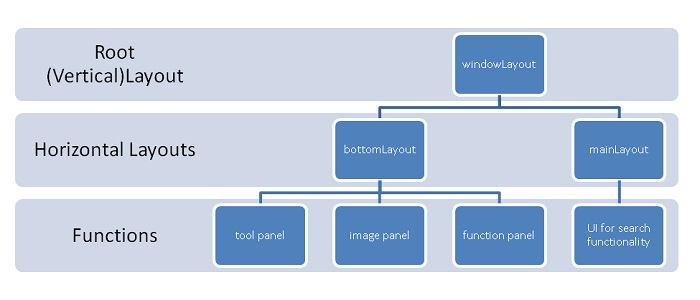
\includegraphics[width=14cm,height=7cm]{layouts.jpg}
\caption{Interface Layout}
\label{fig:1}
\end{figure}

Then the basic search functionality on the basis of issue names,date range was incorporated. Once a issue is selected from the dropdown list and the search button is clicked, all the headlines of the selected issue appears in the table contained in the left pane. And the images of the corresponding issue are displayed in the image panel. The headlines are in the form of links which when clicked shows the entire article in the table itself.

\item In Phase 2, the actual implementation of collaborative text correction tool takes place. Once the entire OCR text is retrieved in the rows of a table, it also gets highlighted in the image at the image panel. If \textgravedbl Edit Text\textasciidieresis button is clicked, the OCR text becomes editable and a save button is displayed at the bottom of the left hand pane. A user can correct the text to match it with the text in the image. \\
After the \textgravedbl Save\textasciidieresis button is clicked, a check is performed against the database to determine which lines of text have been changed.  Only those text lines that have been changed are saved as a new version.
\item In Phase 3, user management functions, advance search options like phrase searching, enhanced UI features and other functionalities of the tool will be focussed.
\end{itemize}

\section{Design Models}
\label{sec:models}
\subsection{Database Design}

The database design of our project is given below.\\

\begin{figure}[ht!]
\centering
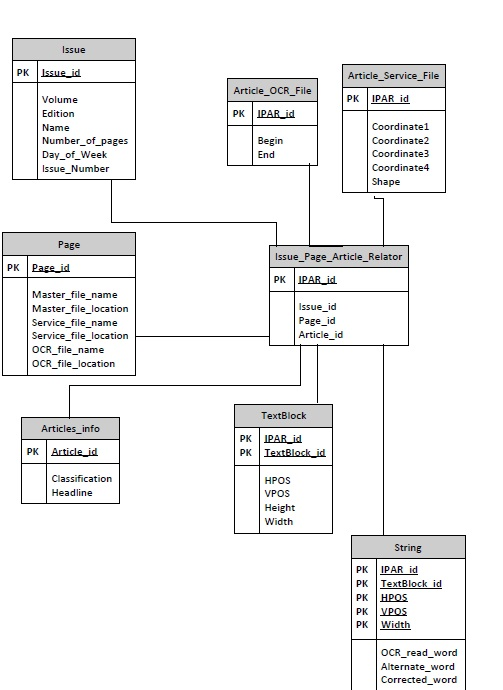
\includegraphics[width=10cm,height=10cm]{diag.jpg}
\caption{Database Design}
\label{fig:2}
\end{figure}

The ER Diagram shown describes the association between the tables present in the database of this project. All the entities are connected to a common entity called \textgravedbl Issue\_Page\_Article\_Relator\textasciidieresis. It contains the primary keys of all other entities. The main entities are \textgravedbl Issue\textasciidieresis that refers to the Newspaper, \textgravedbl Page\textasciidieresis that denotes the pages in the newspaper and Article related entities called \textgravedbl Article\_info\textasciidieresis, \textgravedbl Article\_OCR\_File\textasciidieresis, \textgravedbl Article\_Service\_File\textasciidieresis.\\ \textgravedbl TextBlock\textasciidieresis and \textgravedbl String \textasciidieresis are used to fetch and group all the words in a single article in proper order, hence their attributes include the Horizontal and Vertical position of each textline.\\
Another table was created to save the changes made in the OCR text and to save the user specified tags in the database. This was created due to the challanges faced as mentioned in section~\ref{sec:implementation}.

\begin{figure}[ht!]
\centering
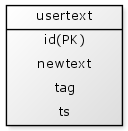
\includegraphics[width=5cm,height=5cm]{entity.jpg}
\caption{Experimental table}
\label{fig:3}
\end{figure}

Here \textgravedbl id\textasciidieresis is bigserial Primary Key, \textgravedbl newtext\textasciidieresis is the user corrected text, \textgravedbl tag\textasciidieresis is the user specified tag corresponding to a given article and \textgravedbl ts\textasciidieresis refers to the timestamp when the insert operation is executed.\\

In this project, Views are used to access the tables present in the database. A View is a virtual table containing fields from one or more real tables. They make information retrieval fast and secure.\\
Following Views are used by the web interface:\\

\begin{tabular}{l|p{10cm}}
\hline
View Name & Description\\
\hline
vw\_issu\_page\_files & \parbox{10cm}{retrieves the page file locations related to particular\\ issue using the \textgravedbl date\_of\_issue\textasciidieresis column}\\
\hline
vw\_issue\_articles & \parbox{10cm}{accesses all the articles related to a particular\\ issue using the \textgravedbl date\_of\_issue\textasciidieresis column}\\
\hline
vw\_image\_info & \parbox{510cm}{accesses the coordinates, shapes and
related data\\ for each article using the \textgravedbl ipar\_id\textasciidieresis column}\\
\hline 
vw\_article\_text & \parbox{10cm}{accesses entire text related to a particular article\\ using the \textgravedbl ipar\_id\textasciidieresis column}\\
 \hline
\end{tabular}

\subsection{Architectural Design}
The architectural style used in this project is the Model-View-Controller (MVC) architecture. MVC is the software architecture pattern that separates the representation of information from user's interaction with it. It is used by applications that need the ability to maintain multiple views of the same data. The interaction between the three components is defined as: \\

\begin{itemize}
\item A controller sends commands to its associated view to change the view's presentation of the model. It can also send commands to the model to update the model's state. It processes every request, prepares other parts of the system like model and view.

\item A model handles data processing and database works part. It processes events sent by controller. After processing these events, it sends processed data to controller (thus, controller may reprocess it) or directly to view side allowing them to produce updated output.

\item A view prepares interface to show to the user.It requests from the model the information that it needs to generate an output representation to the user.\\
\end{itemize}
\begin{figure}[ht!]
\centering
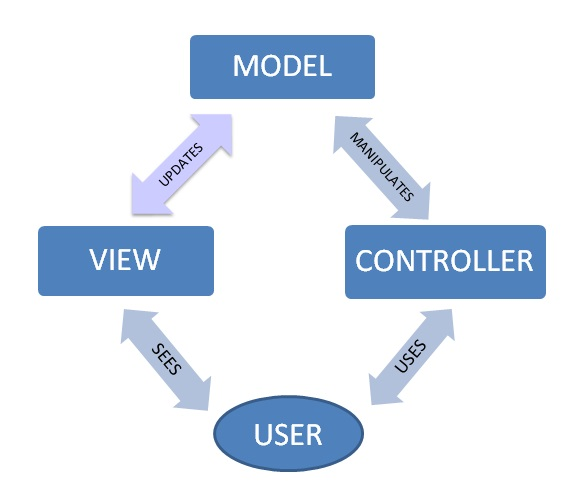
\includegraphics[width=9cm,height=7cm]{mvc1.jpg}
\caption{MVC Architecture}
\label{fig:4}
\end{figure}

\subsubsection{Architectural Description}
In this project, MainWebApp.java is used as the controller which receives calls from the user and calls the relevant screen (model or view) based on the input.\\
IssueDisplay.java acts as a view. This class is the primary display page for an issue, one page at a time.  It takes in the following parameters - list of articles in an issue and the page image to be displayed first.
It then display the list of articles as hyperlinks in the left pane, along with the issue title and display the image in the right pane. \\
DatabaseHelper.java acts as a model contains any database objects that needs representation.


\section{System Study}
\label{sec:system}
\subsection{Hardware Specification}
\begin{itemize}
    \item 32-bit Operating System 
\item 4GB RAM 
\item Intel(R) Core(TM) i3 CPU @ 2.13 GHz
\end{itemize}

\subsection{Software Specification}
\begin{itemize}
\item Eclipse Juno 4.2 IDE \\
It is an Integrated Development Environment (IDE) comprising of a base workspace and an extensible plug-in system for customizing environment. It is used to develop applications primarily in Java and other languages by means of other plug-ins.\\
Vaadin plug-in for eclipse was used to create the web interface of our project.

\item Vaadin 6 (Java Framework) plugin for Eclipse \\
Vaadin is an AJAX web application development framework that enables developers to build high-quality user interfaces with Java, both on the server- and client-side. It provides a set of libraries of ready-to-use user interface components and a clean framework for creating our own components. The focus is on ease-of-use, re-usability, extensibility, and meeting the requirements of large enterprise applications.\\
It is an open source web application for rich Internet applications. It has server side architecture which means that the majority of the logic runs on the server. Ajax technology is used at the browser side to ensure a rich and interactive user experience. On the client-side Vaadin is built on top of Google Web Toolkit (GWT).\\

\item Apache Tomcat 7.0.35
It is an open source web server and servlet container developed by the Apache Software Foundation (ASF). It implements the Java Servlet and the JavaServer Pages (JSP) specifications from Sun Microsystems, and provides a pure Java HTTP web server environment for Java code to run in. \\
It includes tools for configuration and management, but can also be configured by editing XML configuration files.

\item Apache Ant 1.8.4
It is a software tool for automating software build processes. It is similar to \textgravedbl Make\textasciidieresis but is implemented using the Java language, requires the Java platform, and is best suited to building Java projects.\\
The most immediately noticeable difference between Ant and Make is that Ant uses XML to describe the build process and its dependencies, whereas Make uses Makefile format.

\item PostgreSQL
It is an open source object-relational database management system (ORDBMS) available for many platforms including Linux, Microsoft Windows and Mac OS X. \\
It implements the majority of the SQL:2008 standard, is ACID-compliant, is fully transactional (including all DDL statements), has extensible data types, operators, index methods, functions, aggregates, procedural languages, and has a large number of extensions written by third parties.

\item Tortoise SVN 1.7, A Subversion client for Windows
It is a free software that helps programmers manage different versions of the source code for their programs.Tortoise SVN is a Subversion client, implemented as a Microsoft Windows shell extension. It is released under the GNU General Public License.

\item Web Browser, Google Chrome or Mozilla Firefox
\end{itemize}

\subsection{Setting up the code base}
Following are the steps to get the application working:
\begin{enumerate}
\item Checkout the Bodhi Webapps code located here -\\ https://power.ldeo.columbia.edu/svn/Proj/NYPL/Bodhi/Code/WebApps using Twiki username and password.

\item Verify that it has the following directory structure:
\begin{itemize}
    \item build (directory where the classes of some components will be located, for now, this is empty)
\item config (This folder should have two files - log4j.properties and BodhiWebApplication.properties)\\
Edit log4j.properties, change the value for \textgravedbl log4j.appender.A1.File\textasciidieresis to a specific directory on the machine.\\
No changes are required in BodhiWebApplication.properties
\item doc (This is the directory for any documents, including javadoc)
\item resources (If the application is going to use any external resources, they will be stored here)
\item src (Root folder for all the source files)
\item edu.columbia.ccls.dh.bodhi.controller (Folder for all the controllers, these will have the logic to direct the calls to specific components. It will have the code to instantiate the models and views corresponding to the action chosen by the user)
\item edu.columbia.ccls.dh.bodhi.model (Folder for all the model classes, typically any database objects that need representation)
\item edu.columbia.ccls.dh.bodhi.view (Folder for constructing the HTML views. Information needed for constructing will be passed to it by the constructor, typically either an instance of the model or specific values from the model)
\item edu.columbia.ccls.dh.bodhi.utils (Folder for all the utility classes and functions. Components in this folder will be used across the board, like database connections, special string operations, validations.)
\item WebContent (Root folder for all the Vaadin files as well as the web application classes)
\end{itemize}

\item Set up the project in Eclipse, just by choosing create new project from existing source and pointing it to the root folder where the entire folder is checked out.

\item Once the project is created, make sure that the java path is set correctly (it might be different on different machines)

\item Once the project is ready, open the deploy.xml, locate the entry , change the value of the attribute \textgravedbl location \textasciidieresis, point it to the Tomcat installation directory on the machine.

\item Make sure Apache Ant is installed on the machine (if not, download it from apache.org and make sure that the executable location is included in the PATH variable)

\item Verify that there are no errors, then open up a command prompt

\item To connect to the database on Tesla.ldeo.columbia.edu, a tunnel needs to be established. To do this, type \\
ssh -Nn -L 5555:localhost:5432 username@tesla.ldeo.columbia.edu \& \\
Replace the username and password with the corresponding user's name and password.

\item Open another command prompt, change the directory to the root folder of  the project and type ant war. This will compile the project, create a war file and deploy it to the Tomcat's \textgravedbl webapps\textasciidieresis directory.

\item Start Tomcat (if it is not already running), go to bin and run startup.bat to start the server and shutdown.bat to shutdown the server.

\item Open up a web browser, go to http://localhost:8080/bodhi/MainWebApp, to see the page, Bodhi Issue Display created by the application.

\item To verify that the application is up and running correctly, open up the log file that was specified in step number 2
\end{enumerate}


\section{Implementation}
\label{sec:implementation}
\subsection{Functions Implemented}
\begin{enumerate}
\item List of Issues : Populated the combobox with the retrieved list of issues from the database. Illustrated in figure~\ref{fig:5}
\item Article Search : Retrieved articles based on a set of criteria like article topic, issue name, date range. Illustrated in figure~\ref{fig:7}
\item Headlines : Retrieved articles are the headlines in the form of links which when clicked returns the OCR text. Illustrated in figure~\ref{fig:7}
\item Images: Retrieved images of the selected articles in the middle pane.
\item OCR Text : Displayed the raw OCR article text of the user selected headline in the table. Illustrated in figure~\ref{fig:8}
\item OCR Correction  : Raw OCR text can be edited after clicking the \textgravedbl Edit\textasciidieresis button. Once the button is pressed, each row of the table becomes editable. Illustrated in figure~\ref{fig:9}
\item Tag Specification: Interface allows users to specify tags corresponding to the given article which then gets saved into the database. Illustrated in figure~\ref{fig:10}
\item Save corrected Text : Text corrected by the patron gets stored in the database as soon as the \textgravedbl Save\textasciidieresis button is clicked. Illustrated in figure~\ref{fig:11}
\end{enumerate}
	
\subsection{User Interface}
The User Interface is designed using Vaadin. Some of our project screenshots are shown in Appendix A.


\subsection{Remote Debugging Tomcat using Eclipse}
To debug our project, Eclipse Integrated debugger could not be simply used to debug as there was no an executable file. So in order to debug a Tomcat application through Eclipse, following steps need to be taken:
\begin{enumerate}
    \item Open catalina.bat file which can be found in \textgravedbl apache-tomcat-7.0.35/bin/catalina.bat\textasciidieresis
\item Insert two statements after \textgravedbl set CLASSPATH=\textasciidieresis \\
CATALINA\_OPTS=\\
\textgravedbl-Xdebug-Xrunjdwp:transport=dt\_socket,address=8000,server=y,suspend=n\textacutedbl\\
JPDA\_OPTS=\textgravedbl -agentlib:jdwp=transport=dt\_socket,address=8000,server=y,suspend=n\textasciidieresis
\item Save and close the file. 
\item Run Tomcat from command prompt using command: \\
catalina.bat jpda start \\
instead of using the normal startup.bat
\item Then in Eclipse create a debug configuration like below:

\begin{itemize}
    \item Give the project name.
\item Give the connection type as Standard(Socket Attach)
\item Put the host as localhost
\item Specify port as 8000
\item Give any name for configuration.
\end{itemize}

\item After setting the debug configuration, start debugger in Eclipse.
\end{enumerate}
  
\subsection{Challenges}
There were several challenges faced during the project, few of them are listed below.
\begin{enumerate}
\item Firewall at server end: Since the database server was at an external location secured with firewall, there were problems in accessing the server at first.
\item Firewall at client end: After the access was granted the problem arose at my end due to Cyberoam layer. I could access the server from outside but not institution due to restricted remote access in the presence of firewall. Finally I was allotted a port using which I could successfully create a secure tunnel.
\item Inaccessible Images: Images that were to be displayed in the web page were not available publicly as they were present only on the server. So hundreds of images of size 3.5GB were first securely copied (PSCP) to the client and then they were pushed to the cloud.
\item Incompatible Images: All the images that were available were of the format .jp2 which is JPEG 2000. It uses a wavelet compression algorithm instead of the common DCT compression method that is used with standard JPEG images.\\
This format can be used to store either lossy or lossless compressed JPEG images and provides the user with a better quality and smaller file size than the traditional JPG image files.\\
But these images are not supported by the browser, hence they can not be opened in the browser.
\item Performance Issues : Due to the remote access to the server through tunneling and by using complex subquery to retrieve the OCR text, the server got slow. The time clocked for the server to response for the query was 16 minutes when using 3G network. These long delays and other problems made it difficult to work on real data. \\
Query: \\
\textgravedbl select linetext from vw\_ipar\_text1 where ipar\_id IN (select  ipar\_id from vw\_issue\_articles where headline =\textasciidieresis + headline \\
Alternatively,\\
\textgravedbl select linetext from vw\_ipar\_text1 t1 INNER JOIN (select ipar\_id from vw\_issue\_articles where headline =\textasciigrave \textasciidieresis + headline + \textacutedbl\textasciiacute)t2 ON t1.ipar\_id = t2.ipar\_id \textasciidieresis \\
The above queries fetches the entire article corresponding to the user selected headline. But both of them makes the retrieval process slow.\\
So, the functionality to edit the Raw text was built by setting OCR text in the table a priori. And saving the edited data into the database. Section~\ref{sec:models}, figure~\ref{fig:3} defines the table created to save the user corrected text and user specified tags.

\end{enumerate}

\section{Conclusion}
The OCR \cite{OCR} Text Correction System has not been fully implemented yet. There are several challenges as described above that require attention before proceeding further in terms of implementation. This system when functional will contain a repository of articles which would be clean and usable by many. The process of editing text will also help in building and growing of a community.\\
Once the system would be functional, it will certainly act as a rich source of information for historians, researchers, scholars and users in general.\\

\section{Acknowledgement}
This implementation project was a part of my M.Tech Scholarly work. I would like to express my gratitude to both my Advisors Dr. Haimonti Dutta and Manoj Pooleery for their constant support and guidance without which I would have never been able to complete it.

\nocite{cdnc,OCR,eval,noisy,book,eclipse,vaadin,tomcat,ant,postgres,svn,ER}

%\section{Bibiliography}
\bibliography{Scholarly_report}
\bibliographystyle{plain}
\appendix
\appendixpage
\addappheadtotoc

\section{Screenshots}


\begin{figure}[H]
\centering
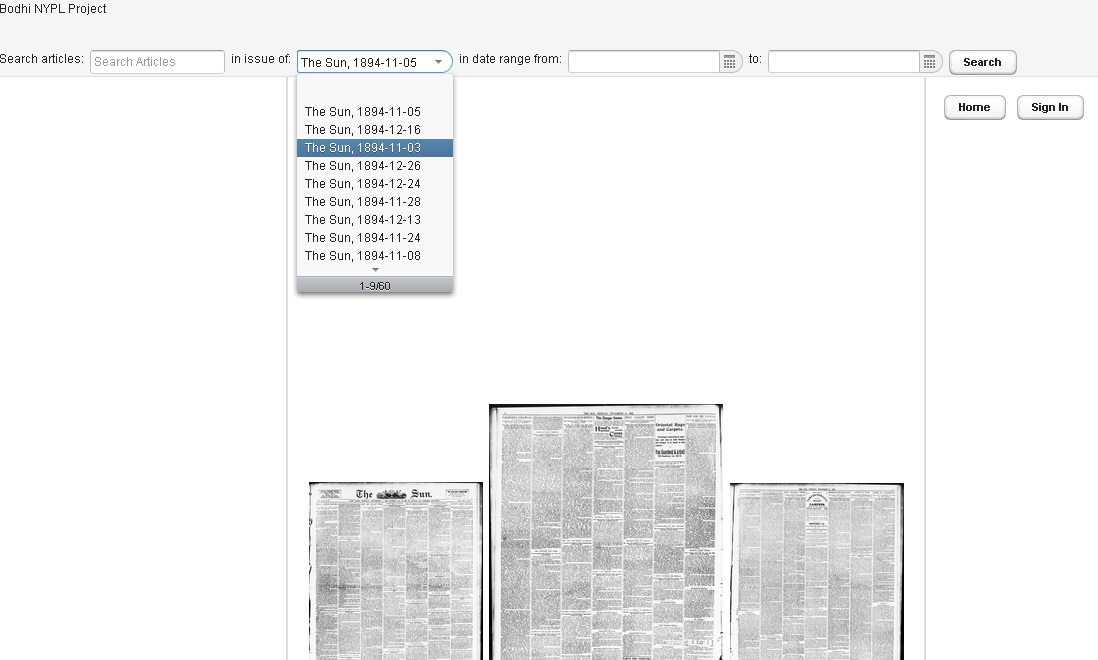
\includegraphics[width=14cm,height=8cm]{dropdown.jpg}
\caption{List of issues}
\label{fig:5}
\end{figure}

\begin{figure}[H]
\centering
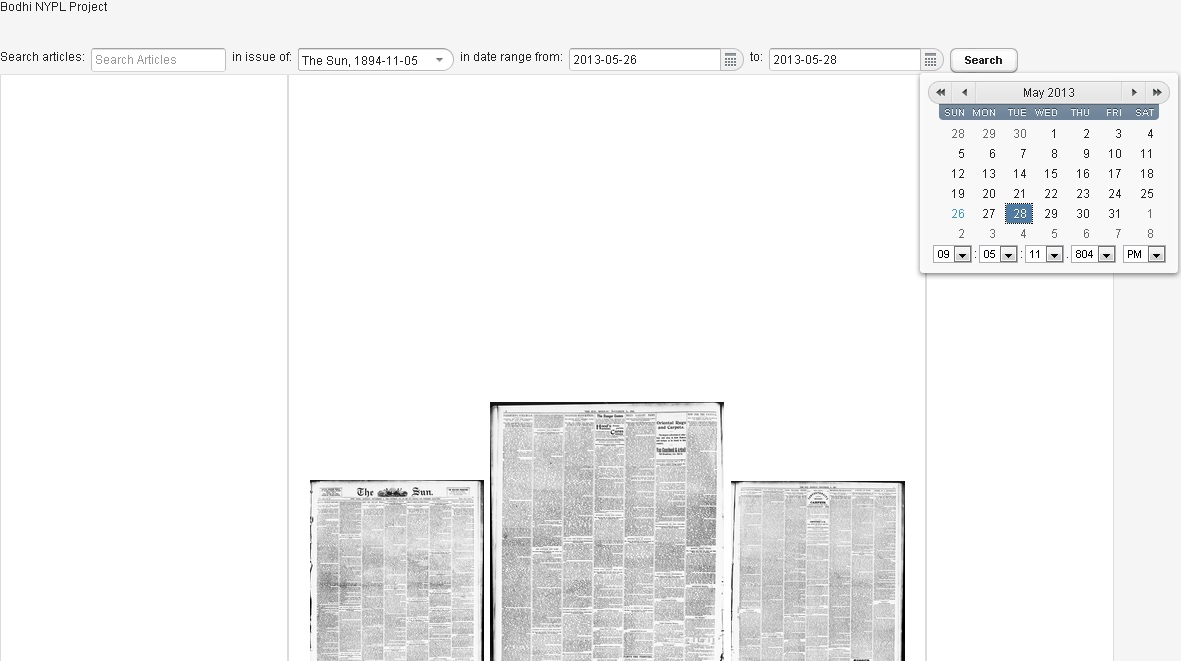
\includegraphics[width=14cm,height=8cm]{datepicker.jpg}
\caption{Datepicker}
\label{fig:6}
\end{figure}

\begin{figure}[H]
\centering
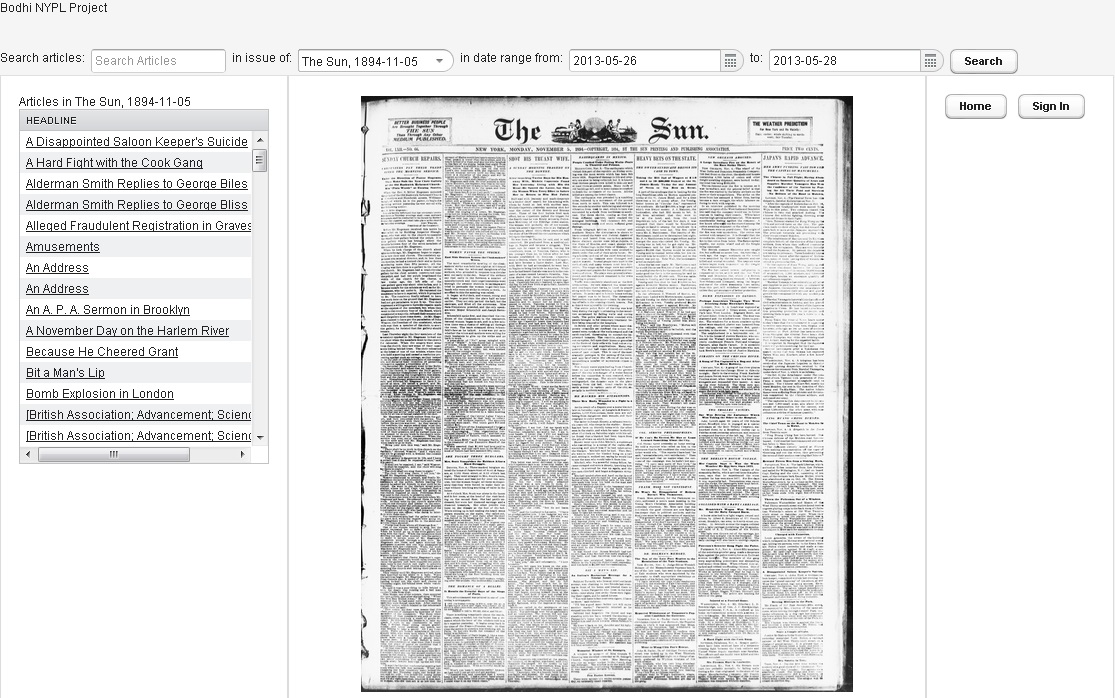
\includegraphics[width=14cm,height=8cm]{results.jpg}
\caption{List of headlines in a issue}
\label{fig:7}
\end{figure}


\begin{figure}[H]
\centering
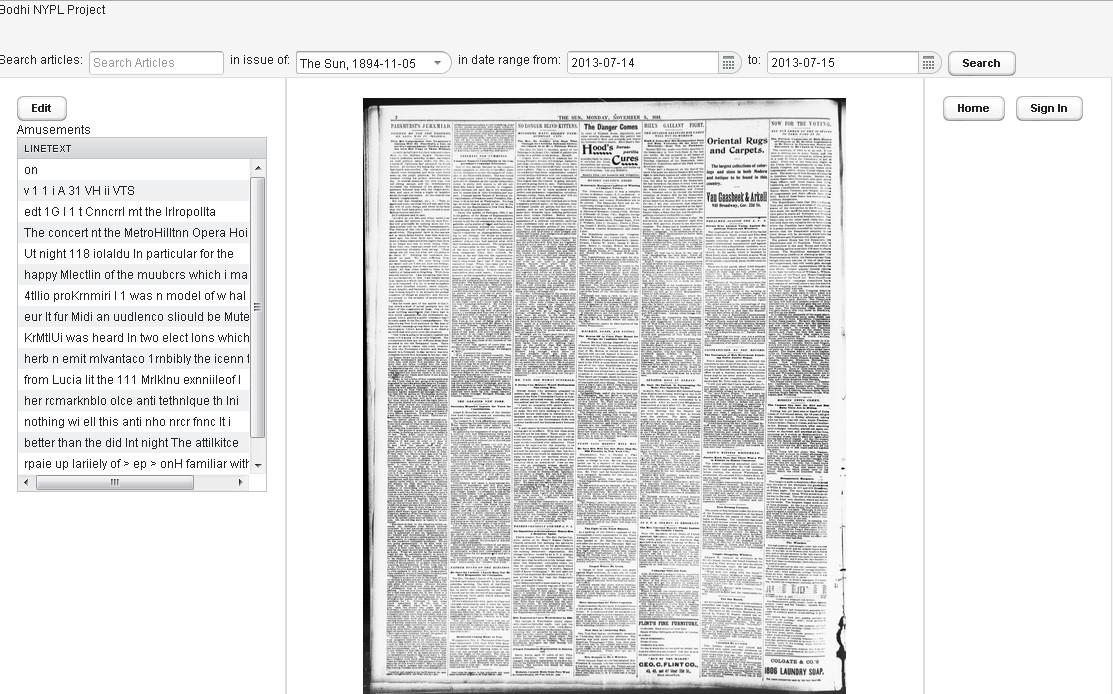
\includegraphics[width=14cm,height=8cm]{beforeEditText.jpg}
\caption{OCR Text of the headline \textasciigrave Amusements\textasciiacute}
\label{fig:8}
\end{figure}

\begin{figure}[H]
\centering
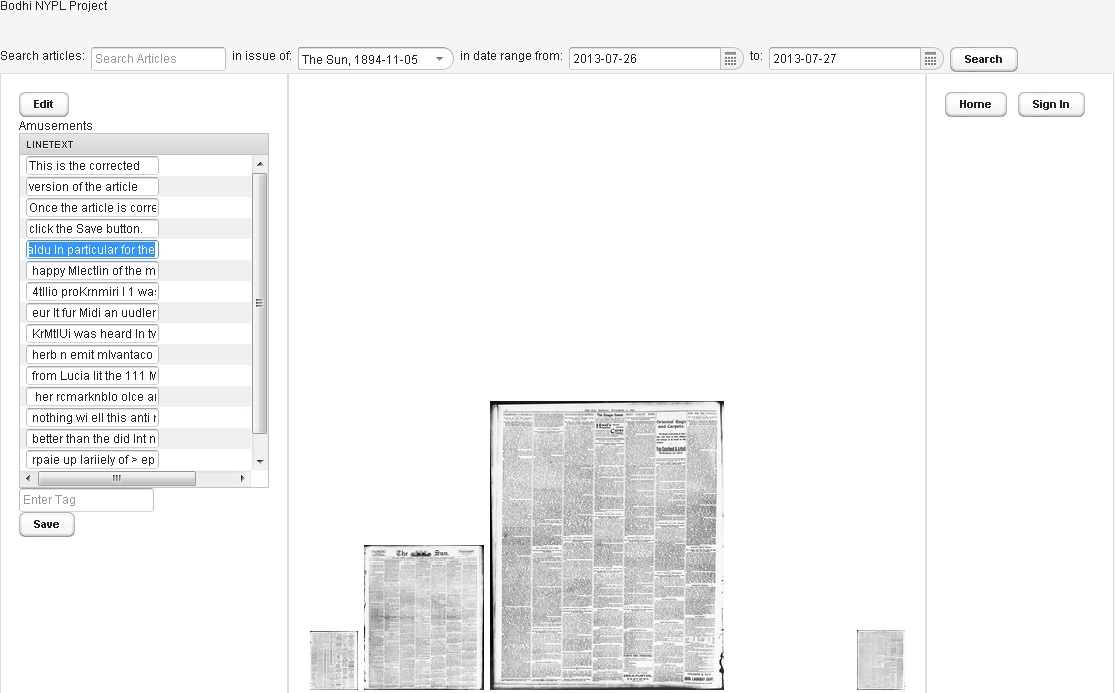
\includegraphics[width=14cm,height=8cm]{editing.jpg}
\caption{Editing the Raw Text}
\label{fig:9}
\end{figure}

\begin{figure}[H]
\centering
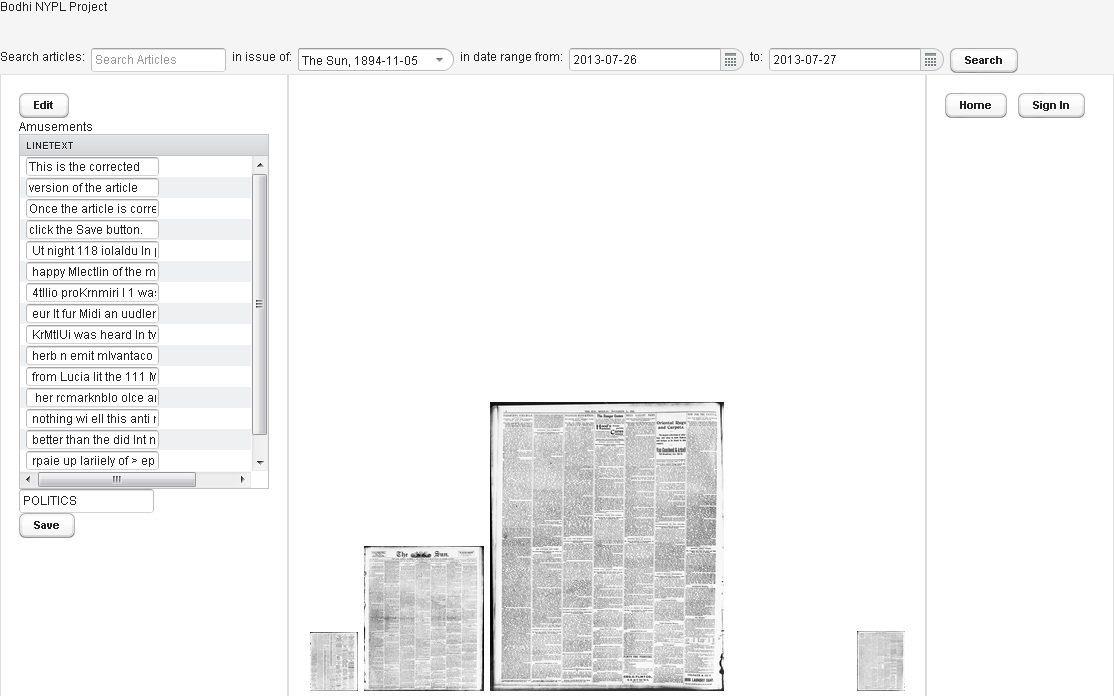
\includegraphics[width=14cm,height=8cm]{tag.jpg}
\caption{User Specified Tag}
\label{fig:10}
\end{figure}

\begin{figure}[H]
\centering
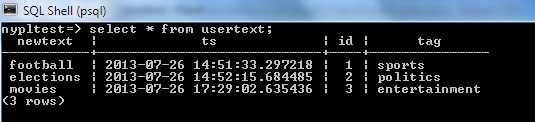
\includegraphics[width=9cm,height=4cm]{db.jpg}
\caption{Snapshot of the table}
\label{fig:11}
\end{figure}

\end{document}













